\chapter{Tensor networks, entanglement, and controlled computation}
\label{ch:tensor_networks}

Exact diagonalization exposes the finite spectrum directly, but its state
space grows exponentially. Matrix product states trade the full wavefunction
for a structured variational family whose cost is governed by a bond
dimension. To use them for the Haagerup problem, we must preserve fusion-path
constraints and distinguish physical correlation lengths from symmetry-cat
effects. This chapter introduces the essential tensor algebra, derives the
transfer-matrix and entropy diagnostics, and explains what a converged
finite-bond calculation can establish. The final section treats resource
estimates as part of the mathematical design of an algorithm.

\section{Compressing a wavefunction by successive Schmidt decompositions}
\index{Schmidt decomposition}\index{matrix product state}

For a bipartite pure state,
\[
 |\Psi\rangle=\sum_{a=1}^D\sqrt{p_a}\,
       |a\rangle_L|a\rangle_R,
 \qquad p_a\geq0,\quad\sum_ap_a=1.
\]
The Schmidt rank counts the independent correlations crossing the cut.
To obtain this decomposition, write the wavefunction coefficients in
product bases as a matrix $M_{ij}$. Its singular-value decomposition
$M=U\Sigma V^\dagger$ gives orthonormal left and right vectors and
nonnegative singular values $\Sigma_{aa}=\sqrt{p_a}$. The right
Schmidt vector has coefficients $\overline{V_{ja}}$ in this
convention. Tracing over either side leaves eigenvalues $p_a$;
the eigenvectors on the two sides need not resemble the original
product bases.

Successive Schmidt decompositions along an open chain produce a matrix
product representation
\[
 \Psi(s_1,\ldots,s_L)
 =A^{s_1}_1A^{s_2}_2\cdots A^{s_L}_L,
\]
with boundary vectors understood. Every finite state admits such a
representation, but the exact bond dimensions can grow exponentially.
An MPS approximation restricts these dimensions.

\begin{figure}[htbp]
\centering
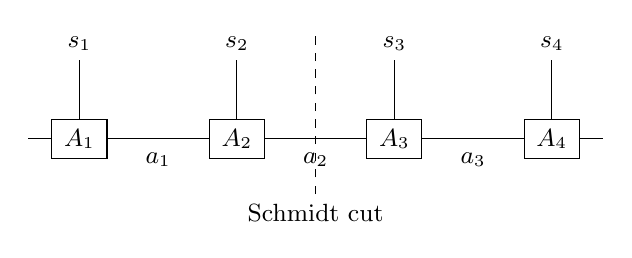
\begin{tikzpicture}[every node/.style={font=\small}]
 \draw (-.65,0)--(6.65,0);
 \foreach \x/\s in {0/1,2/2,4/3,6/4} {
   \draw[fill=white] (\x-.35,-.25) rectangle (\x+.35,.25);
   \node at (\x,0) {$A_{\s}$};
   \draw (\x,.25)--(\x,1);
   \node[above] at (\x,1) {$s_{\s}$};
 }
 \node[below] at (1,-.05) {$a_1$};
 \node[below] at (3,-.05) {$a_2$};
 \node[below] at (5,-.05) {$a_3$};
 \draw[dashed] (3,-.7)--(3,1.35);
 \node[below] at (3,-.7) {Schmidt cut};
\end{tikzpicture}
\caption{Physical indices point upward; horizontal virtual indices are
contracted. The virtual dimension at a cut bounds its Schmidt rank.
In a constrained edge MPS the virtual space is further organized by
the fusion height.}
\label{fig:MPS-cut}
\end{figure}

If one truncates a single Schmidt decomposition to the largest $D$
probabilities and renormalizes, the squared overlap with the original
state is $\sum_{a\leq D}p_a$. This is an exact one-cut statement. A long
variational calculation involves many cuts, changing bases, and an
optimization over tensors; a discarded weight reported at one update
is not automatically the global ground-state error.

The one-cut truncation is optimal for a precise reason. Any normalized
state of Schmidt rank at most $D$ lies in $W\otimes\HH_R$ for
some left subspace $W$ of dimension at most $D$. If $P_W$ is its
projector, Cauchy--Schwarz bounds its overlap with $\Psi$ by
$\|(P_W\otimes1)\Psi\|$. The square of this norm is
$\Tr(P_W\rho_L)$, maximized by the $D$ largest eigenvalues of
$\rho_L$. The normalized truncated Schmidt state attains the bound.
Writing $\varepsilon=\sum_{a>D}p_a$, its fidelity is $1-\varepsilon$
and its phase-aligned squared vector error is
$2-2\sqrt{1-\varepsilon}$. These are different error conventions.

\begin{example}[A bond restriction changes the variational minimum]
For two qubits, let
$|\Phi\rangle=(|00\rangle+|11\rangle)/\sqrt2$ and
$H=-|\Phi\rangle\langle\Phi|$. Both Schmidt probabilities are
$1/2$. Every normalized product state therefore has squared overlap
at most $1/2$ with $\Phi$, so its energy is at least $-1/2$.
A bond-two state represents $\Phi$ exactly and reaches the true
ground energy $-1$. A perfectly converged bond-one optimization
would still miss half the binding energy. Convergence within a
variational family and accuracy of that family are separate issues.
\end{example}

For a uniform periodic MPS,
\begin{equation}
 \Psi(s_1,\ldots,s_L)=\Tr(A^{s_1}\cdots A^{s_L}),
 \label{eq:ordinary-MPS}
\end{equation}
the same tensor is used at every site. The trace enforces cyclic
invariance of the amplitude. It does not require the state to be a
unique ground state or to have finite correlation length.

There is a gauge freedom
$A^s\mapsto X^{-1}A^sX$, which telescopes inside the trace. Overall
rescaling changes the unnormalized state by a length-dependent scalar
and leaves normalized expectation values unchanged. Optimizing raw
coordinates without accounting for these directions can create
ill-conditioned Hessians and misleading gradient norms.

\section{An exact fusion-compatible ansatz}

The path basis suggests a more economical object. Assign a virtual
space $V_a$ of dimension $D_a$ to each height $a$, and a matrix
\[
 W_{ab}:V_b\longrightarrow V_a
\]
to every allowed edge $a\to b$. Set $W_{ab}=0$ on forbidden edges.
The periodic amplitude is
\begin{equation}
 \Psi(x_0,\ldots,x_{L-1})
 =\Tr\bigl(W_{x_0x_1}W_{x_1x_2}\cdots W_{x_{L-1}x_0}\bigr).
 \label{eq:edge-MPS}
\end{equation}
Every nonzero amplitude is an admissible fusion path. No penalty term is
needed to enforce the constraint. Heightwise gauges
$W_{ab}\mapsto X_a^{-1}W_{ab}X_b$ again telescope.

The ansatz can be embedded in an ordinary MPS on the six-state height
space. On $V=\bigoplus_aV_a$, define $A^a$ to have only its $a$th block
row nonzero, with $(a,b)$ block $W_{ab}$. A product of such tensors
forces the intermediate block indices to match the physical height
word, and its trace is exactly \eqref{eq:edge-MPS}. This bridge allows
ordinary MPS results to be applied after the relevant support and
redundant virtual directions are understood.

One can instead work in the full height-spin tensor product and add a
positive energy penalty for forbidden edges. That is another legitimate
variational scheme, but constraint leakage becomes an observable that
must be monitored. Small energy changes do not guarantee small leakage.
For a constrained Hamiltonian, an exactly admissible ansatz has a
particularly transparent variational interpretation.

\begin{example}[Why a product of edge weights is already correlated]
Take $D_a=1$, so every allowed $W_{ab}$ is a scalar. The amplitude is
then a product of nearest-neighbor factors, but it is generally not an
ordinary product state: each physical height occurs in two neighboring
factors. Its squared norm is the partition function of a one-dimensional
classical transfer matrix $K_{ab}=|W_{ab}|^2$. This is the simplest
nontrivial constrained MPS and will reappear in the exact module
construction of Chapter~\ref{ch:gapped}.
\end{example}

\section{What one variational update actually solves}
\index{variational update}

The variational principle says that a normalized admissible state has
energy at least the true ground energy. It does not say that the
nonlinear energy function of all MPS tensors has a single minimum.
A common strategy holds every tensor except one fixed. Collect that
tensor's allowed entries into a vector $a$. The many-body state then
depends linearly on $a$:
\[
 |\Psi(a)\rangle=\sum_\mu a_\mu|v_\mu\rangle.
\]
The environment vectors $v_\mu$ need not be orthogonal or linearly
independent. Their Gram and Hamiltonian matrices are
\[
 N_{\mu\nu}=\langle v_\mu|v_\nu\rangle,\qquad
 H^{\rm eff}_{\mu\nu}=\langle v_\mu|H|v_\nu\rangle.
\]
Consequently the energy is a generalized Rayleigh quotient,
\[
 E(a)=\frac{a^\dagger H^{\rm eff}a}{a^\dagger Na}.
\]
Varying with respect to $\overline a$ at fixed norm gives
\begin{equation}
 H^{\rm eff}a=E Na.
 \label{eq:MPS-local-update}
\end{equation}
The lowest solution minimizes the energy in this linear update
space. If $N$ has a kernel, those coordinates represent the zero
physical state and must first be removed. On its positive support,
$b=N^{1/2}a$ converts the problem to the ordinary Hermitian matrix
$N^{-1/2}H^{\rm eff}N^{-1/2}$.

\begin{example}[Why the norm environment cannot be dropped]
Use the preceding two-qubit Hamiltonian and the nonorthogonal update
basis $v_1=|00\rangle$, $v_2=|\Phi\rangle$. Direct inner products give
\[
 N=\begin{pmatrix}1&1/\sqrt2\\1/\sqrt2&1\end{pmatrix},
 \qquad H^{\rm eff}=-\begin{pmatrix}1/2&1/\sqrt2\\1/\sqrt2&1\end{pmatrix}.
\]
The generalized eigenpair $a=(0,1)^T$, $E=-1$ is the exact
ground state. The orthogonal physical state has coordinates
$a=(\sqrt2,-1)^T$ and energy zero. Diagonalizing $H^{\rm eff}$
alone would instead give eigenvalues $-3/2$ and zero. The spurious
value lies below the Hamiltonian's lowest eigenvalue: it is a
coordinate-norm error, not an improved variational state.
\end{example}

On an open chain, successive Schmidt gauges can make the left and
right environments orthonormal at the update site; then $N=1$ on
the retained support. Periodic and uniform formulations generally
retain nontrivial environments or enforce their fixed-point equations.
The edge ansatz additionally restricts updates to allowed height
blocks, so every vector in the update space remains admissible.

The exact linear-update argument treats site tensors as independent
variables. In a strictly uniform ansatz, changing the shared tensor
changes every site simultaneously, so the global state is no longer
linear in its entries. A uniform algorithm's local effective equation
must be combined with consistent environments and the full uniform
stationarity condition. It cannot be justified by silently treating
all the other copies of the same variable as fixed.

A sweep repeats these local minimizations. Each exact unrestricted
one-tensor update cannot raise the energy, but the final point can
still be a local stationary point of the full nonlinear problem.
A two-tensor update can change the intermediate Schmidt support;
its subsequent truncation can raise the energy again. Neither a
small local residual nor a small coordinate gradient bounds the
missing directions outside the chosen bond dimensions. Independent
initializations, increasing variational support, energy variance,
and a stable set of physical observables answer different parts
of that accuracy question.

The effective matrices in \eqref{eq:MPS-local-update} need not be
stored densely. Their action on a trial tensor can be contracted
through environments. This is the link between the variational
derivation and the resource discussion below: the mathematical
Rayleigh quotient does not prescribe a dense allocation.

\section{Transfer operators and correlation lengths}
\index{transfer map}

For the ordinary tensor \eqref{eq:ordinary-MPS}, define the completely
positive transfer map
\[
 \mathcal E(X)=\sum_sA^sX(A^s)^\dagger.
\]
Completely positive means that
$\mathrm{id}_{M_r(\C)}\otimes\mathcal E$ preserves positive
semidefinite matrices for every auxiliary dimension $r$.
The displayed formula has this property because each summand acts
as $Z\mapsto(1\otimes A^s)Z(1\otimes A^s)^\dagger$.
A transfer map need not preserve the ordinary matrix trace.
Suppose its leading eigenvalue is simple and positive. Rescale the
tensors so this eigenvalue is one, and choose right and left fixed
matrices $r,l\geq0$ with
\[
 \mathcal E(r)=r,\qquad \mathcal E^*(l)=l,\qquad \Tr(lr)=1.
\]
An inserted physical operator $O$ gives
\[
 \mathcal E_O(X)=\sum_{s,t}\langle s|O|t\rangle
          A^tX(A^s)^\dagger,
\]
and its infinite-chain expectation is
$\langle O\rangle=\Tr[l\mathcal E_O(r)]$.
This specifies the stationary infinite-chain state associated with
the chosen fixed metrics. A unique clustering limit of periodic
rings additionally needs the primitive component discussed below;
a simple leading eigenvalue alone does not exclude other peripheral
roots.

For separated one-site insertions,
\[
 \langle O_0P_n\rangle
 =(l|\mathcal E_O\mathcal E^{n-1}\mathcal E_P|r),
\]
using Hilbert--Schmidt bra-ket notation. Subtracting the fixed-point
projector $\mathcal P=|r)(l|$ removes the product of means. An
eigenvalue $\lambda=|\lambda|e^{ik}$ below the unit circle contributes
an exponentially decaying oscillation
$|\lambda|^ne^{ikn}$. Its length and wave number are
\begin{equation}
 \xi_\lambda=-\frac1{\log|\lambda|},\qquad k_\lambda=\arg\lambda.
 \label{eq:MPS-correlation-length}
\end{equation}
Polynomial factors can accompany Jordan blocks, but do not change the
leading exponential rate.

The longest transfer length need not occur in every correlation
function. A source can have zero overlap with that transfer eigenmode
by symmetry. Thus a length extracted from a particular local observable
and the largest length in a computed transfer sector need not coincide.
A partial transfer eigensolve should be described as a spectrum among
the retained modes, not as a complete periphery certificate.

\subsection{Primitivity, periodicity, and cats}
\index{primitivity!transfer map}

A primitive transfer map has an algebraically simple leading
eigenvalue, no other eigenvalues of the same modulus, and strictly
positive fixed metrics on its minimal support. Merely having one
distinct peripheral eigenvalue is insufficient: the identity map
on matrices has only the eigenvalue $1$, with a large eigenspace.
A primitive map describes
a clustering pure phase in the usual injective MPS setting. Two
different mechanisms can spoil the naive use of
\eqref{eq:MPS-correlation-length}.

First, a direct sum of inequivalent injective tensors describes a
superposition of distinct phases. The transfer has more than one
stationary block. A symmetric cat of ordered phases has vanishing
one-point order but nonzero long-distance order correlations. Second,
a tensor can be irreducible but periodic, with peripheral roots of
unity. A three-cycle produces roots $1,e^{2\pi i/3},e^{-2\pi i/3}$.
Neither phenomenon is evidence for a critical connected correlation
length.
After blocking $p$ sites, a subleading blocked eigenvalue measures
$\xi=-p/\log|\lambda_{\rm blocked}|$ in original lattice sites.

\begin{example}[A three-state cat]
Let $|o_j\rangle=|j\rangle^{\otimes L}$ for three orthonormal
one-site states $|j\rangle$, with $L\ge2$. These ordered product
states are cycled by alpha. Let the local order operator $M$ have
values $m\omega^j$ on them, with
$\omega=e^{2\pi i/3}$. In the normalized symmetric cat,
$\langle M\rangle=0$, but
\[
 \langle M_0^\dagger M_n\rangle=|m|^2
\]
at every separation. The infinite apparent length measures mixing of
ordered components. In any individual component the connected
correlator is zero. A tiny finite-bond splitting of a cat transfer
root can produce an enormous but physically inappropriate number
from \eqref{eq:MPS-correlation-length}.
\end{example}

For the Haagerup variational sequence, primitive-component and
intraphase transfer restrictions are therefore part of the observable
definition. Raw near-unit roots cannot simply be fed into an entropy
fit. Equivalent redundant tensor blocks are another possibility: they
can multiply peripheral eigenvalues without representing different
physical vacua. One must distinguish a minimal state decomposition
from the displayed virtual dimension.

\section{Schmidt probabilities from the fixed metrics}

For an injective ordinary MPS in the thermodynamic limit, the nonzero
Schmidt probabilities are the eigenvalues of
\[
 \sigma=\sqrt l\,r\sqrt l,
 \qquad\Tr\sigma=1,
\]
in a consistent virtual convention. A gauge transformation changes
the metrics but not these probabilities. Replacing the expression by
the diagonal entries of $r$, or by eigenvalues of a tensor block
without its left metric, generally gives the wrong entropy.

The entropies are
\[
 S_1=-\sum_ap_a\log p_a,\qquad
 S_n=\frac1{1-n}\log\sum_ap_a^n,
 \qquad S_\infty=-\log p_{\max}.
\]
For a cat, one must specify whether the full cat entropy or the
entropy of one primitive component is being used. For components with
mutually orthogonal Schmidt supports on both sides of the cut and
classical weights $w_j$, the von Neumann entropy includes
the mixing entropy $-\sum_jw_j\log w_j$ as well as the component
entropies averaged with weights $w_j$. For general R\'enyi order the
block-diagonal density matrix instead gives
\[
 S_n=\frac1{1-n}\log\left(\sum_jw_j^n\Tr\rho_j^n\right),
\]
where $\rho_j$ is the normalized reduced state of component $j$.
The mixing contribution is real, but it is not the entanglement
of a single clustering vacuum.

In a constrained height representation, a cut can retain coherent
boundary-charge information. Pinching the reduced density matrix into
height sectors, weighting those sectors by quantum dimensions, and
taking the ordinary Schmidt spectrum are three different operations.
The entropy convention must be fixed before comparing ranks or models.

\section{Why entropy measures the central charge}
\label{sec:MPS-replica}
\index{replica trick}\index{twist field!replica}\index{entanglement entropy}

The coefficient in an entropy fit comes from the stress-tensor anomaly.
We can derive it using the Schwarzian transformation law of
Chapter~\ref{ch:cft}. Consider the vacuum of a unitary full CFT on the
infinite line, with $c_L=c_R=c$, and an interval $A=[u,v]$ of length
$\ell=v-u$. Keep a microscopic cutoff $a$ so that its reduced density
matrix is well defined. For an integer $n\geq2$, multiplying $n$ copies
of this density matrix and tracing joins the copies cyclically along
$A$. The resulting Euclidean surface has $n$ sheets, with branch
points at $u$ and $v$.

Equivalently, use $n$ copies of the CFT on one plane and insert fields
$\mathcal T_n(u)$ and $\widetilde{\mathcal T}_n(v)$ that implement
the cyclic permutation and its inverse. The stress tensor in this
replica theory is the sum $T^{\rm tot}=\sum_{j=1}^nT_j$, with chiral
central charge $nc$. The branch geometry is uniformized by
\[
 z(w)=\left(\frac{w-u}{w-v}\right)^{1/n}.
\]
Different sheets choose different phases of this root. Those phases
do not change its Schwarzian derivative. The vacuum stress in the
$z$ plane vanishes, so on each sheet
\[
 \langle T_j(w)\rangle=\frac c{12}\{z,w\}.
\]
To evaluate it, write $g(w)=(w-u)/(w-v)$. A direct differentiation
gives $\{g,w\}=0$ and
$\{g^{1/n},g\}=(1-n^{-2})/(2g^2)$. The Schwarzian chain rule then
gives
\[
 \langle T^{\rm tot}(w)\rangle
 =\frac c{24}\left(n-\frac1n\right)
   \frac{(u-v)^2}{(w-u)^2(w-v)^2}.
\]
On the other hand, the Ward identity for two conjugate primaries of
weight $h_n$ gives exactly the same rational function with coefficient
$h_n$. We have therefore calculated the replica weights:
\begin{equation}\label{eq:MPS-twist-weight}
 \begin{aligned}
 h_n=\bar h_n&=\frac c{24}\left(n-\frac1n\right),\\
 \Delta_n=2h_n&=\frac c{12}\left(n-\frac1n\right).
 \end{aligned}
\end{equation}
The factor $n$ in the total stress is essential. Using only one
sheet's stress would miss it.

The twist two-point function now determines the interval moment:
\[
 \Tr\rho_A^n=C_n(\ell/a)^{-2\Delta_n},\qquad C_1=1.
\]
The constants $C_n$ depend on the cutoff convention. Substitution in
the definition of the R\'enyi entropy gives
\begin{equation}\label{eq:MPS-interval-Renyi}
 S_n(A)=\frac c6\left(1+\frac1n\right)\log(\ell/a)+k_n.
\end{equation}
Here $k_n=\log C_n/(1-n)$ records the nonuniversal constant.
The physical continuation near $n=1$ is the one defined by powers of
the regulated positive density matrix. It yields
$S_1=(c/3)\log(\ell/a)+k_1$. Integer replica values by themselves
are not an abstract uniqueness theorem for analytic continuation.
For a periodic spatial circle of circumference $L$, the plane-to-cylinder
map replaces $\ell$ by the chord length:
\[
 S_n(\ell,L)=\frac c6\left(1+\frac1n\right)
 \log\left[\frac L{\pi a}\sin\frac{\pi\ell}{L}\right]+k_n.
\]
This uses the conformal vacuum on the circle. A finite lattice has
additional corrections to the scaling formula.

A half-infinite bipartition has one entangling endpoint. To obtain
a finite entropy, consider a clustering massive vacuum near the
critical point, with one large length $\xi$. Its replica moment is a
single twist expectation. Scaling gives
\[
 \Tr\rho_{\rm half}^n
   \sim A_n(a/\xi)^{\Delta_n},\qquad
 S_n^{\rm half}
   =\frac c{12}\left(1+\frac1n\right)\log(\xi/a)+s_n+o(1).
\]
Here $A_n$ depends on the massive theory and regulator. The power uses
one twist dimension, whereas an interval two-point function uses two.
This explains the factor of two between the two geometries. Replacing
this physical correlation length by the length of a finite-bond MPS
is a further scaling hypothesis, considered in the next section.

\begin{example}[Ising entropies and an ordered cat]
For the Ising CFT, $c=1/2$. The logarithmic coefficients of
$S_1,S_2,S_\infty$ on an interval are respectively
$1/6,1/8,1/12$; the corresponding single-cut coefficients are
$1/12,1/16,1/24$. The last values use the regime in which the
scaling formula also controls the largest Schmidt probability.
A common factor-of-two error would turn the correct Ising
single-cut von Neumann slope $1/12$ into a spurious estimate
$c=1/4$ if one used the interval coefficient $c/3$.

The three-component product-state cat considered above instead has
$\Tr\rho_A^n=3^{1-n}$ across a nontrivial cut, hence $S_n=\log3$
for every $n$. Its entropy has no logarithmic length slope. More
generally, suppose three components have mutually orthogonal Schmidt
supports on both sides of the cut, the same Schmidt probabilities
$p_a$, and equal weights. The full probabilities are
$p_a/3$, each repeated three times. Thus
$S_n^{\rm cat}=S_n^{\rm component}+\log3$. A fixed mixing constant
does not change an asymptotic slope; changing component weights
along a variational sequence can change a finite entropy secant.

Global orthogonality of the components alone would not suffice.
For instance the three qutrit states
$|\Phi_j\rangle=3^{-1/2}\sum_{a=0}^2\zeta_3^{ja}|a,a\rangle$
are orthonormal and each has three equal Schmidt probabilities.
Yet their normalized equal superposition is $|0,0\rangle$, a
product state. Their Schmidt supports overlap; the preceding
ordered-cat formula uses the stronger support condition explicitly.
\end{example}

\section{Finite-entanglement scaling as a hypothesis to test}
\index{finite-entanglement scaling}

A finite-bond MPS approximation to a critical ground state often acts
as an infrared regulator. Under the usual single-scale critical
assumptions, the half-chain Rényi entropy behaves as
\begin{equation}
 S_n=\frac c{12}(1+1/n)\log\xi+s_n+\cdots.
 \label{eq:FES}
\end{equation}
Thus adjacent entropy secants are converted to central-charge
diagnostics with factors $6,8,12$ for $n=1,2,\infty$. All orders
should use the same pair of tensors and the same physically specified
correlation length. Mixing an entropy from one checkpoint with a
length from a later optimization has no reason to obey the formula.

If a symmetry-breaking finite-bond state has a local order amplitude
$|m|\sim\xi^{-\Delta}$ for one dominant scaling field, then
\[
 \Delta_{\rm eff}
 =-\frac{\log(|m_b|/|m_a|)}{\log(\xi_b/\xi_a)}.
\]
There is no factor of one half unless the observable used is
$|m|^2$. Several microscopic order sources can have different finite
slopes because their subleading mixtures differ.

\begin{numericalrecord}[The present stationary sequence]
In the completed October 5 record, the largest checkpoint qualified
by the unchanged stationarity test has rank parameter $144$,
energy density approximately $-.84533646847$, and component
transfer length approximately $154.8613$ sites.
Three consecutive accepted coordinate gradients and a fresh uncached
same-point check pass the threshold $10^{-6}$; the latter gives
$7.67\times10^{-7}$. The rank-$156$ trial reaches the lower energy
$-.84533724589$, but its gradient $6.27\times10^{-5}$ fails the
same criterion and it is excluded from the qualified sequence.

The newest adjacent conditional entropy estimates are
\[
 \begin{array}{c|ccc}
 \text{rank pair}&c_1&c_2&c_\infty\\ \hline
 120\text{--}132&2.75608&2.65579&2.35197\\
 132\text{--}144&1.55824&1.59321&1.47876
 \end{array}
\]
The comparison retains all $28$ contiguous rank windows.
A fit through the four checkpoints of ranks $108,120,132,144$
gives $c_1=2.09890$. Its proximity to two does not make the
strongly varying adjacent slopes a plateau. Stationarity
qualifies the variational data for comparison; it does not
establish the single-scale conformal assumptions of
\eqref{eq:FES} or a continuum error bound.
\end{numericalrecord}

Here the saved rank parameter $r$ labels height-fiber dimensions
$D_{I_j}=r$ and $D_{X_j}=3r$. The cyclic implementation further
splits them into three phase blocks of dimensions $r/3$ and $r$.
Thus rank parameter $144$ does not mean that the full ordinary
embedding has bond dimension $144$; its block structure is part
of the tensor definition and of the resource estimate.

The lower variational energy at a larger rank is useful even when its
entropy has not converged. It does not justify mixing that point into
a qualified scaling sequence. Conversely, a strict coordinate-gradient
gate is an optimization criterion, not a physical approximation-error
bound. A high-quality sequence should retain energy, independent
gradient checks, variance, transfer residuals, primitive-component
tests, and entropies at the same tensors.

There is a second possible interpretation of growing $\xi$: a model
with a very large but finite physical correlation length may look
critical until the variational regulator exceeds that scale. Failure
to see saturation at current ranks does not prove a divergent exact
length. The gapped alternatives of the next chapter make this
possibility especially relevant.

\section{Energy variance and the transfer resolvent}

For $H_L=\sum_jh_j$ in a clustering translation-invariant state,
\begin{equation}
 \lim_{L\to\infty}\frac{\operatorname{Var}(H_L)}L
 =\langle h_0^2\rangle-e^2
 +2\sum_{r\geq1}\Re\bigl(\langle h_0h_r\rangle-e^2\bigr),
 \label{eq:variance-density}
\end{equation}
provided the connected series is summable. Here $e=\langle h\rangle$.
For $h=-P_\rho$, $h^2=-h$, so the coincident term is $-e-e^2$.
Overlapping adjacent terms must be handled separately; their ordered
product is not necessarily Hermitian, although the full variance is
real.

The distant tail can be summed without enumerating separations. On
the centered transfer subspace,
\[
 \sum_{n=0}^{\infty}(\mathcal E-\mathcal P)^n
 =(1-\mathcal E+\mathcal P)^{-1}.
\]
Applying this reduced resolvent to a centered insertion vector turns
the infinite sum into a linear equation. It can be solved through
matrix-free Krylov methods, which repeatedly apply $\mathcal E$ but
never store its dense matrix. The stationary direction is explicitly
removed; otherwise the inverse is singular.

The variance density is an independent variational diagnostic. For
an exact eigenstate on a finite ring it vanishes. A small density in
an infinite ansatz does not by itself bound its fidelity with a
particular ground state, because that requires spectral information.
It also does not decide whether a decreasing variational energy
sequence approaches a critical state or a massive one.

\section{Local correlators and disconnected plateaus}

An ordered MPS can be useful for testing proposed fields, but its
long-distance raw moments include its mean. For a charged density
$O$ with $\langle O\rangle=m$, clustering gives
\[
 \langle O_0^\dagger O_r\rangle\to|m|^2,\qquad
 \langle O_0O_rO_{2r}\rangle\to m^3.
\]
The absolute normalized triple-to-pair ratio therefore approaches one,
irrespective of an intermediate-distance CFT coefficient. Averaging
over an ordered cat removes $\langle O\rangle$ but can retain these
plateaus. Component centering and connected cumulants answer a
different question from averaging over all symmetry-related vacua.

A possible scaling window must satisfy two competing inequalities:
the separation is much larger than the operator support and
microscopic scale, but much smaller than the variational or physical
correlation length. At currently available bond dimensions that
window can be narrow. Period-three oscillations also require
demodulation or separate residue classes. A smooth ratio at a few
separations is a diagnostic; it does not establish its universal
limit.

The same issue arises for energy structure factors. If the local
energy density really approaches $v(T+\bar T)/(2\pi)$, the
nonanalytic small-momentum part is proportional to $cv^2|q|^3$.
Analytic contact terms, density improvements, finite transfer length,
and higher powers can coexist. Cancelling a fitted analytic term
does not remove every omitted correction, and an estimate of $cv^2$
still requires a velocity to become an estimate of $c$.

\section{Designing a calculation whose resources are understood}

A useful tensor identity can be computationally unusable in its
literal form. An ordinary bond-$D$ transfer matrix has $D^2$ rows and
$D^2$ columns, hence $D^4$ entries. Complex double precision uses
$16D^4$ bytes for that matrix alone. Its input tensor, copies,
factorizations, and a solver workspace may coexist with it.

The danger is not hypothetical in this project: an older optimization
path contained approximately $468D^4$ complex entries in one hidden
workspace, about $47.18$ GiB at $D=51$, before other live objects.
Inspecting only the allocating wrapper would have missed an in-place
call that created the workspace. The correct object to audit is the
actual execution path.

Matrix-free contractions often replace a $D^4$ storage cost by a
small number of $D^2$ vectors and $D^3$ arithmetic steps, although
the exact exponents depend on the tensor structure. Fusion-height
blocks and cyclic phase blocks can reduce both constants and powers.
Streaming one endpoint pair or one local contraction at a time avoids
holding all intermediates together. A reduced-resolvent solve should
use a bounded Krylov restart rather than an unbounded stored basis.

\begin{example}[Why ``small bond rank'' can be misleading]
A categorical line can enlarge each height fiber by summing over
fusion-compatible incoming fibers. In the actual rho-line lift, a
rank pair $(r,3r)$ becomes $(3r,10r)$. A coherent direct sum with the
original tensor has ranks $(4r,13r)$. Even if the original $r$ looks
small, forming a dense transfer matrix of the full ordinary embedding
can already exceed desktop memory by orders of magnitude. The
height-block representation, not the nickname of the original rank,
determines the allocation.
\end{example}

A peak estimate should count simultaneously live basis arrays,
operator tables, Krylov vectors, coordinate/gradient copies, library
workspaces, decompression buffers, and cache charged to the job. A
read-only checkpoint consumer can have small resident arrays but
substantial file-cache use. Swap is not an additional compute
budget: paging a memory-exhausted eigensolve can make a shared desktop
unusable even without an immediate allocation failure.

For reproducing calculations on the project machine, the canonical
machine policy and its central guarded launcher govern admission,
memory reservations, CPU affinity, and thread counts. Historical
commands in research notes are provenance, not current permission
to reuse an old larger budget. A research method should degrade
gracefully: reuse checkpoints, work in a smaller sector, stream a
contraction, or prove an algebraic statement when safe numerical
admission is unavailable.

\section{Exercises}

\begin{exercise}\label{ex:MPS-schmidt}
Take the normalized two-qutrit state
$|\Psi\rangle=\sqrt{1/2}|00\rangle+\sqrt{1/3}|11\rangle+
\sqrt{1/6}|22\rangle$ and $H=-|\Psi\rangle\langle\Psi|$.
Find the normalized optimal Schmidt-rank-two approximation,
its fidelity, its vector-norm error, and its energy. Compare
with the best rank-one energy. Explain why allowing arbitrary
local basis changes cannot improve these optima.

\par\smallskip\noindent{\footnotesize\normalfont
\hyperref[sol:ex:MPS-schmidt]{Solution on page~\pageref*{sol:ex:MPS-schmidt}.}}\par
\end{exercise}
\begin{exercise}\label{ex:MPS-edge}
Verify that the block-row ordinary tensor constructed from $W_{ab}$
has periodic amplitude \eqref{eq:edge-MPS}. Identify the virtual
index constraints imposed by multiplying two consecutive tensors.

\par\smallskip\noindent{\footnotesize\normalfont
\hyperref[sol:ex:MPS-edge]{Solution on page~\pageref*{sol:ex:MPS-edge}.}}\par
\end{exercise}
\begin{exercise}\label{ex:MPS-correlation}
For the scalar-edge family with three colors, real $t$, and
$W_t(i,j)=t$ when $i=j$ and $1$ otherwise, compute the norm-transfer
eigenvalues and the nontrivial correlation length. Analyze $t=0$,
$t=1$, and large $|t|$.

\par\smallskip\noindent{\footnotesize\normalfont
\hyperref[sol:ex:MPS-correlation]{Solution on page~\pageref*{sol:ex:MPS-correlation}.}}\par
\end{exercise}
\begin{exercise}\label{ex:MPS-cat}
Compute the ordinary bipartite entropy of the three-component
product-state cat in the example. Explain why a nonzero entropy
constant and long-range order do not imply a nonzero central charge.

\par\smallskip\noindent{\footnotesize\normalfont
\hyperref[sol:ex:MPS-cat]{Solution on page~\pageref*{sol:ex:MPS-cat}.}}\par
\end{exercise}
\begin{exercise}\label{ex:MPS-resolvent}
Starting from the transfer expression for separated correlators,
derive the centered geometric series and its reduced resolvent.
State what fails when another eigenvalue has modulus one.

\par\smallskip\noindent{\footnotesize\normalfont
\hyperref[sol:ex:MPS-resolvent]{Solution on page~\pageref*{sol:ex:MPS-resolvent}.}}\par
\end{exercise}
\begin{exercise}\label{ex:MPS-scaling}
Derive the conversion factors $6,8,12$ from \eqref{eq:FES}.
Suppose $S_1=a\log\xi+b+u/\log\xi$. Compute the effective secant
between two lengths and explain why a slowly drifting slope need
not have reached its limiting value.

\par\smallskip\noindent{\footnotesize\normalfont
\hyperref[sol:ex:MPS-scaling]{Solution on page~\pageref*{sol:ex:MPS-scaling}.}}\par
\end{exercise}
